\input{../../../.preambles/02-lab_work}
\usepackage{epstopdf}
\newgeometry{top=1.5cm, bottom=1.5cm, left=1cm, right=1cm}
\begin{document}
    \begin{table}[h!]
        \center
        \begin{tabular}{|C{.5}|C{.2}|C{.25}|}
            \hline
            \multicolumn{1}{|c|}{\multirow{4}{*}{Лабораторная работа № 4}} &
            Студент, группа & {{ student }}, Ф-369 \\ \cline{2-3}
            & Дата выполнения & 02.03.2013 \\ \cline{2-3}
            & Подпись &  \\ \cline{2-3}
            Исследование характеристик & Дата отчёта & \\ \cline{2-3}
            электронно-лучевой трубки & Оценка &  \\ \cline{2-3}
            & Подпись &  \\ \hline
        \end{tabular}
    \end{table}

    \emph{Цель работы:} Ознакомиться с принципом работы, конструкциями и
    характеристиками электронно-лучевых трубок (ЭЛТ).
    
    \begin{table}[h!]
        \center
        \caption{Зависимость смещения луча по горизонтали от величины
        отклоняющего напряжения}
        \begin{tabular}{|C{.08}|*{13}{C{.045}|}} \hline
            \( X \), мм & -30 & -25 & -20 & -15 & -10 & -5 & 0 & 5 & 10 & 15
            & 20 & 25 & 30 \\ \hline
            \( U_1 \), В & -64,5 & -53,2 & -43,2 & -32,4 & -22,2 & -10,7 & 0,0
            & 11,2 & 21,3 & 32,9 & 43,6 & 53,6 & 64,5 \\ \hline
            \( U_2 \), В & -65,9 & -54,5 & -43,8 & -32,4 & -21,3 & -10,3 & 0,3
            & 10,8 & 22,2 & 32,8 & 43,0 & 54,2 & 64,8 \\ \hline
            \( U_3 \), В & -66,1 & -55,4 & -44,2 & -33,3 & -22,0 & -10,4 & 0,1
            & 11,2 & 22,4 & 33,8 & 44,7 & 54,8 & 65,3 \\ \hline
            \( \midnum{U} \), В & -65,5 & -54,4 & -43,7 & -32,7 & -21,8 & -10,5
            & 0,1 & 11,1 & 22,0 & 33,2 & 43,7 & 54,2 & 64,9 \\ \hline
        \end{tabular}
    \end{table}
    
    \begin{table}[h!]
        \center
        \caption{Зависимость смещения луча по вертикали от величины
        отклоняющего напряжения}
        \begin{tabular}{|C{.08}|*{13}{C{.045}|}} \hline
            \( Y \), мм & -30 & -25 & -20 & -15 & -10 & -5 & 0 & 5 & 10 & 15
            & 20 & 25 & 30 \\ \hline
            \( U_1 \), В & -52,3 & -43,8 & -35,6 & -24,8 & -15,7 & -8,8 & 0,2
            & 8,8 & 16,7 & 24,5 & 33,7 & 41,4 & 49,6 \\ \hline
            \( U_2 \), В & -52,4 & -44,3 & -35,4 & -25,3 & -16,3 & -9,6 & 0,3
            & 9,7 & 15,1 & 24,3 & 32,8 & 41,6 & 50,5 \\ \hline
            \( U_3 \), В & -50,9 & -44,5 & -35,3 & -25,7 & -19,2 & -9,1 & 0,7
            & 7,8 & 15,2 & 23,4 & 32,8 & 41,6 & 50,2 \\ \hline
            \( \midnum{U} \), В & -51,9 & -44,2 & -35,4 & -25,3 & -17,1 & -9,2
            & 0,4 & 8,8 & 15,7 & 24,1 & 33,8 & 41,9 & 50,1 \\ \hline
        \end{tabular}
    \end{table}
    
    \begin{table}[h!]
        \center
        \caption{Зависимость катодного тока от напряжения на модуляторе}
        \begin{tabular}{|C{.064}|*{12}{C{.05}|}} \hline
            \( J_K \),~мкА & -11,35 & -11,03 & -10,90 & -10,70 & -10,60 & -10,30
            & -9,36 & -7,05 & 0,00 & 2,66 & 20,10 & 39,80 \\ \hline
            \( U_M \), В & -67,3 & -65,0 & -64,0 & -62,4 & -61,7 & -59,6 & -55,3
            & -50,7 & -46,3 & -45,4 & -40,8 & -37,2 \\ \hline
        \end{tabular}
    \end{table}
    
    \begin{table}[h!]
        \center
        \caption{Результаты}
        \begin{tabular}{|*{6}{C{.145}|}} \hline
            Чувствительность \( D_x \) & Погрешность измерений \( \Delta_x \) &
            Чувствительность \( D_y \) & Погрешность измерений \( \Delta_y \) &
            Потенциал запирания \( U_\emph{з} \) & Погрешность измерений
            \( \Delta_J \) \\ \hline
            0,46 & & 0,59 & &  & \\ \hline
        \end{tabular}
    \end{table}
    \emph{Вывод:}
\begin{figure}
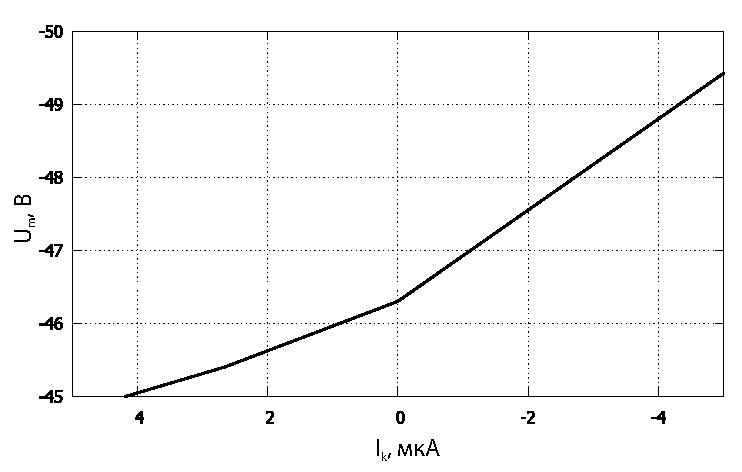
\includegraphics[width=\textwidth]{j}
\end{figure}
\end{document}
